\documentclass[12pt]{report}
\usepackage{graphicx}     %Note graphics<graphicx<epsfig
\usepackage[table,xcdraw, dvipsnames]{xcolor}
\usepackage{hyperref} %written by Sebastian Rahtz
%\usepackage{subeqn}    %allows equations 1a, 1b
%\usepackage{subfig}    %allows figures 1a, 1b
\usepackage{amsmath}
\usepackage{amssymb}
\usepackage{xurl}
\usepackage{bbm}%for indicator function
%\bibliographystyle{alpha}
\usepackage{floatrow}
\usepackage[normalem]{ulem}
\usepackage{tikz}
\usepackage{xparse, expl3, istgame, makecell}



\usepackage{tocloft}

%\usepackage{emoji}

% Adjust number widths
\setlength{\cftchapnumwidth}{2em}
\setlength{\cftsecnumwidth}{3.2em}
\setlength{\cftsubsecnumwidth}{3.5em}

\usepackage[toc,page]{appendix}
\usepackage[nottoc]{tocbibind}

\usepackage[color,matrix,frame,arrow,curve]{xy}
\usepackage[shortlabels]{enumitem}
\usepackage{array}
\usepackage{pdflscape}
\usepackage{multicol, multirow}
\usepackage{ctable}
\usepackage{dirtree}
\usepackage{subfig}
\usepackage{longtable}
\usepackage{pdfpages}
\usepackage{esvect}

\usepackage{bm}

%\usepackage{fdsymbol}
%\usepackage{animate}% play animation

\usepackage[vlined,ruled]{algorithm2e}
\newcommand{\mycommfont}[1]{\small\ttfamily\textcolor{blue}{#1}}
\SetCommentSty{mycommfont}

%highlighting
\usepackage{mdframed}

\usepackage[makeroom]{cancel}

\usepackage{pdfpages}
\usepackage{hyperxmp}
\usepackage{tensor}

% this escapes the underscore in text
%\usepackage[T1]{fontenc}
%\usepackage{underscore}

\paperheight=11in
\topmargin=0in
\headheight=0in
\headsep=0in
\topskip=0in
\textheight=8.5in
\footskip=.5in


\paperwidth=8.5in
\oddsidemargin=.25in
\evensidemargin=.25in
\textwidth=6.0in
\parindent=.5in

\newcommand{\bcen}[0]{\begin{array}{c}}
\newcommand{\ecen}[0]{\end{array}}
\newcommand{\twoarrows}[0]{\uparrow\downarrow}
\newcommand{\circone}{\tiny (1)}


\newcommand{\chapquote}[3]{\begin{quotation} \textit{#1} \end{quotation} \begin{flushright} - #2, \textit{#3}\end{flushright} }

\newtheorem{claim}{Claim}
\newcommand{\proof}[0]{{\bf proof:} }
\newcommand{\qed}[0]{\quad\newline \noindent{\bf QED }}

\newcommand{\upto}[0]{-}
\newcommand{\XT}[2]{{\substack{#1\\#2}}}

\newcommand{\bra}[1]{\langle#1|}
\newcommand{\ket}[1]{|#1\rangle}
\newcommand{\av}[1]{\left\langle#1\right\rangle}
\newcommand{\pder}[2]{\frac{\partial#1}{\partial#2}}
\newcommand{\der}[2]{\frac{d#1}{d#2}}
\newcommand{\tr}[0]{{\rm tr }}
\newcommand{\beq}{\begin{equation}}
\newcommand{\eeq}{\end{equation}}
\newcommand{\bsub}{\begin{subequations}}
	\newcommand{\esub}{\end{subequations}}
\newcommand{\beqa}{\begin{eqnarray}}
\newcommand{\eeqa}{\end{eqnarray}}
\newcommand{\rarrow}[0]{\rightarrow}
\newcommand{\larrow}[0]{\leftarrow}
\newcommand{\uarrow}[0]{\uparrow}
\newcommand{\darrow}[0]{\downarrow}
\newcommand{\Rarrow}[0]{\Rightarrow}
\newcommand{\nRarrow}[0]{\nRightarrow}
\newcommand{\Larrow}[0]{\Leftarrow}
\newcommand{\nLarrow}[0]{\nLeftarrow}
\newcommand{\ul}[1]{\uline{#1}}
\newcommand{\ol}[1]{\overline{#1}}
\newcommand{\CC}[0]{{ \mathbb{C}} }
\newcommand{\EE}[0]{{ \mathbb{E}} }
\newcommand{\FF}[0]{{ \mathbb{F}} }
\newcommand{\GG}[0]{{ \mathbb{G}} }
\newcommand{\NNN}[0]{ {\mathbb{N}}} %\NN already defined
\newcommand{\PP}[0]{{ \mathbb{P}} }
\newcommand{\RR}[0]{{ \mathbb{R}} }
\newcommand{\TT}[0]{{ \mathbb{T}} }
\newcommand{\WW}[0]{ {\mathbb{W}}}
\newcommand{\XX}[0]{{ \mathbb{X}} }
\newcommand{\YY}[0]{{ \mathbb{Y}} }
\newcommand{\ZZ}[0]{ {\mathbb{Z}}}

\renewcommand{\Re}{{\rm Re}}
\renewcommand{\Im}{{\rm Im}}



\newcommand{\ground}{{}_{\stackrel{\stackrel{\displaystyle{\bot}}{-}}{.}}}
\newcommand{\norm}[1]{\parallel#1\parallel}
\newcommand{\eqdef}[0]{\;\;\stackrel{\text{def}}{=}\;\;}

\newcommand{\heavy}[0]{\mathbf{H}}

\newcommand{\rva}[0]{{\ul{a}}}
\newcommand{\rvb}[0]{{\ul{b}}}
\newcommand{\rvc}[0]{{\ul{c}}}
\newcommand{\rvd}[0]{{\ul{d}}}
\newcommand{\rve}[0]{{\ul{e}}}
\newcommand{\rvf}[0]{{\ul{f}}}
\newcommand{\rvg}[0]{{\ul{g}}}
\newcommand{\rvh}[0]{{\ul{h}}}
\newcommand{\rvi}[0]{{\ul{i}}}
\newcommand{\rvj}[0]{{\ul{j}}}
\newcommand{\rvk}[0]{{\ul{k}}}
\newcommand{\rvl}[0]{{\ul{l}}}
\newcommand{\rvll}[0]{{\ul{\ell}}}
\newcommand{\rvm}[0]{{\ul{m}}}
\newcommand{\rvn}[0]{{\ul{n}}}
\newcommand{\rvo}[0]{{\ul{o}}}
\newcommand{\rvp}[0]{{\ul{p}}}
\newcommand{\rvq}[0]{{\ul{q}}}
\newcommand{\rvr}[0]{{\ul{r}}}
\newcommand{\rvs}[0]{{\ul{s}}}
\newcommand{\rvt}[0]{{\ul{t}}}
\newcommand{\rvu}[0]{{\ul{u}}}
\newcommand{\rvv}[0]{{\ul{v}}}
\newcommand{\rvw}[0]{{\ul{w}}}
\newcommand{\rvx}[0]{{\ul{x}}}
\newcommand{\rvy}[0]{{\ul{y}}}
\newcommand{\rvz}[0]{{\ul{z}}}


\newcommand{\rvA}[0]{{\ul{A}}}
\newcommand{\rvB}[0]{{\ul{B}}}
\newcommand{\rvC}[0]{{\ul{C}}}
\newcommand{\rvD}[0]{{\ul{D}}}
\newcommand{\rvE}[0]{{\ul{E}}}
\newcommand{\rvF}[0]{{\ul{F}}}
\newcommand{\rvG}[0]{{\ul{G}}}
\newcommand{\rvH}[0]{{\ul{H}}}
\newcommand{\rvI}[0]{{\ul{I}}}
\newcommand{\rvJ}[0]{{\ul{J}}}
\newcommand{\rvK}[0]{{\ul{K}}}
\newcommand{\rvL}[0]{{\ul{L}}}
\newcommand{\rvM}[0]{{\ul{M}}}
\newcommand{\rvN}[0]{{\ul{N}}}
\newcommand{\rvO}[0]{{\ul{O}}}
\newcommand{\rvP}[0]{{\ul{P}}}
\newcommand{\rvQ}[0]{{\ul{Q}}}
\newcommand{\rvR}[0]{{\ul{R}}}
\newcommand{\rvS}[0]{{\ul{S}}}
\newcommand{\rvT}[0]{{\ul{T}}}
\newcommand{\rvU}[0]{{\ul{U}}}
\newcommand{\rvV}[0]{{\ul{V}}}
\newcommand{\rvW}[0]{{\ul{W}}}
\newcommand{\rvX}[0]{{\ul{X}}}
\newcommand{\rvY}[0]{{\ul{Y}}}
\newcommand{\rvZ}[0]{{\ul{Z}}}

\newcommand{\rvbeta}[0]{{\ul{\beta}}}
\newcommand{\rvxi}[0]{{\ul{\xi}}}
\newcommand{\rvzeta}[0]{{\ul{\zeta}}}
\newcommand{\rvtheta}[0]{{\ul{\theta}}}
\newcommand{\rvmu}[0]{{\ul{\mu}}}
\newcommand{\rvsig}[0]{{\ul{\sigma}}}
\newcommand{\rvDel}[0]{{\ul{\Delta}}}
\newcommand{\rvtau}[0]{{\ul{\tau}}}

\newcommand{\cala}[0]{{\cal A}}
\newcommand{\calb}[0]{{\cal B}}
\newcommand{\calc}[0]{{\cal C}}
\newcommand{\cald}[0]{{\cal D}}
\newcommand{\cale}[0]{{\cal E}}
\newcommand{\calf}[0]{{\cal F}}
\newcommand{\calg}[0]{{\cal G}}
\newcommand{\calh}[0]{{\cal H}}
\newcommand{\cali}[0]{{\cal I}}
\newcommand{\calk}[0]{{\cal K}}
\newcommand{\call}[0]{{\cal L}}
\newcommand{\calm}[0]{{\cal M}}
\newcommand{\caln}[0]{{\cal N}}
\newcommand{\calo}[0]{{\cal O}}
\newcommand{\calp}[0]{{\cal P}}
\newcommand{\calq}[0]{{\cal Q}}
\newcommand{\calr}[0]{{\cal R}}
\newcommand{\cals}[0]{{\cal S}}
\newcommand{\calt}[0]{{\cal T}}
\newcommand{\calu}[0]{{\cal U}}
\newcommand{\calv}[0]{{\cal V}}
\newcommand{\calw}[0]{{\cal W}}
\newcommand{\calx}[0]{{\cal X}}
\newcommand{\caly}[0]{{\cal Y}}
\newcommand{\calz}[0]{{\cal Z}}

%\newcommand{\diamante}[1]{\Big\langle#1\Big\rangle}
\newcommand{\diamante}[1]{*++[F=]{#1}}
%\newcommand{\corchete}[1]{\Big\{#1\Big\}}
\newcommand{\corchete}[1]{#1}
\newcommand{\cuadro}[1]{*++[F]{#1}}

\newcommand{\Pmat}[4]{\calp\left[
\begin{array}{cc}#1&#2\\#3&#4
\end{array}\right]}

%\newcommand{\PN}[0]{PN^{0,0}_{1,1}}
%\newcommand{\PS}[0]{PS^{1,1}_{0,0}}
\newcommand{\PN}[0]{PN}
\newcommand{\PS}[0]{PS}

\newcommand{\lam}[0]{\lambda}
\newcommand{\Lam}[0]{\Lambda}
\newcommand{\alp}[0]{\alpha}
\newcommand{\eps}[0]{\epsilon}
\newcommand{\s}[0]{\sigma}
\newcommand{\su}[0]{{\Sigma}}

\newcommand{\pp}[0]{\mathbb{P}}
\newcommand{\dbm}[0]{{
		[1,\partial_{b},\partial_{m}]
}}

\newcommand{\dg}[0]{{[1, \partial_{\theta_G}]}}
\newcommand{\dd}[0]{{[1, \partial_{\theta_D}]}}
\newcommand{\dgd}[0]{{[1, \partial_{\theta_G}, \partial_{\theta_D}]}}

\newcommand{\veca}[0]{{\vec{a}}}
\newcommand{\vecb}[0]{{\vec{b}}}
\newcommand{\vecc}[0]{{\vec{c}}}
\newcommand{\vecd}[0]{{\vec{d}}}
\newcommand{\vecf}[0]{{\vec{f}}}
\newcommand{\vech}[0]{{\vec{h}}}
\newcommand{\vecr}[0]{{\vec{r}}}
\newcommand{\vecs}[0]{{\vec{s}}}
\newcommand{\vecu}[0]{{\vec{u}}}
\newcommand{\vecx}[0]{{\vec{x}}}
\newcommand{\vecy}[0]{{\vec{y}}}
\newcommand{\vechy}[0]{{\vec{\haty}}}
\newcommand{\vtheta}[0]{{\vec{\theta}}}

\newcommand{\haty}[0]{{\widehat{y}}}
\newcommand{\hatx}[0]{{\widehat{x}}}
\newcommand{\hata}[0]{{\widehat{a}}}
\newcommand{\hatr}[0]{{\widehat{r}}}


\newcommand{\cond}[0]{{\:\mathbf{|}\:}}
\newcommand{\mymathbf}[1]{#1}

\newcommand{\ranvec}[1]{\ul{\vec{#1}}}
\newcommand{\indi}[0]{\mathbbm{1}}
\newcommand{\smoid}[0]{{\rm smoid}}
\newcommand{\lodds}[0]{{\rm lodds}}
\newcommand{\expit}[0]{{\rm expit}}
\newcommand{\logit}[0]{{\rm logit}}
\newcommand{\sign}[0]{{\rm sign}}

\renewcommand{\labelitemii}{$\bullet$}

\newcommand{\HAT}[1]{{\widehat{#1}}}
\newcommand{\TIL}[1]{{\widetilde{#1}}}
\newcommand{\tild}[0]{{\TIL{d}}}
\newcommand{\tile}[0]{{\TIL{e}}}
\newcommand{\tilg}[0]{{\TIL{g}}}
\newcommand{\tilu}[0]{{\TIL{u}}}
\newcommand{\tilx}[0]{{\TIL{x}}}
\newcommand{\tilP}[0]{{\TIL{P}}}
\newcommand{\tilPT}[0]{{\TIL{P}_\theta}}

\newcommand{\maparrow}[1]
{\xymatrix{\ar[r]_{#1}&}}


\newcommand{\ucalm}[0]{\ul{\calm}}

\newcommand{\bool}[0]{\{0,1\}}

\newcommand{\argmin}{\mathop{\mathrm{argmin}}\limits}
\newcommand{\argmax}{\mathop{\mathrm{argmax}}\limits}

\newcommand{\softmax}[0]{{\rm softmax}}

\newcommand{\A}[0]{\wedge}
\newcommand{\V}[0]{\vee}
\newcommand{\xor}{\oplus}
\newcommand{\bigA}[0]{\bigwedge}
\newcommand{\bigV}[0]{\bigvee}
\newcommand{\bigxor}{\bigoplus}


\newcommand{\rdart}[0]{\Rightarrow}
\newcommand{\ldart}[0]{\Leftarrow}
\newcommand{\rveps}[0]{\ul{\eps}}

\newcommand{\hatvar}[0]{\widehat{\sigma^2}}
\newcommand{\ptp}[0]{{(t)}}

\newcommand{\tseries}[1]{{\{#1\}_{\forall t}}}

\newcommand{\xbeta}[0]{X_\s^T\beta}
\newcommand{\xtau}[0]{X_\s^T\tau}

\newcommand{\LeafAr}[1]{
\ar@{->}@/_1pc/[#1]
\ar@{<-}@/^1pc/[#1]
}
\newcommand{\Rect}[1]{*++[F-]{#1}}
\newcommand{\Circle}[1]{*++[o][F-]{#1}}
\newcommand{\DCircle}[1]{*++[o][F=]{#1}}
\newcommand{\PinkCircle}[1]{*++[o][F-][F**:pink]{#1}}
\newcommand{\PinkDCircle}[1]{*++[o][F=][F**:pink]{#1}}

\newcommand{\OTO}[0]{\boxed{\bf \checkmark OTO}\;}
\newcommand{\COTO}[0]{\boxed{\bf \checkmark OTO}\;}

%\xymatrix{
%&a
%\\
%\DCircle{\rvx}\LeafAr{ru}&
%}

%https://tex.stackexchange.com/questions/208905/loops-of-different-sizes

\newcommand{\loopup}[2]{ % \ar@(ul,ur) size is like 3
\ar@`{[]+/ul+#1pc/,[]+/ur+#1pc/}#2[]}
\newcommand{\loopdown}[2]{ % \ar@(ul,ur) size is like 3
\ar@`{[]+/dl+#1pc/,[]+/dr+#1pc/}#2[]}
\newcommand{\loopright}[2]{ % \ar@(ul,ur) size is like 3
\ar@`{[]+/dr+#1pc/,[]+/ur+#1pc/}#2[]}
\newcommand{\loopleft}[2]{ % \ar@(ul,ur) size is like 3
\ar@`{[]+/dl+#1pc/,[]+/ul+#1pc/}#2[]}

% test code
%\xymatrix{
%\rva\loopup{3}{@[green]_r}
%&
%\rvb\loopdown{3}{@[red]_r}
%&
%\rvc\loopright{3}{@[blue]_r}
%\\
%\rvd\loopleft{3}{@[violet]_r}
%}


\newcommand{\redminus}[0]{{\color{red}\bm{\;-\;}}} 
\newcommand{\redplus}[0]{{\color{red}\bm +}}
\newcommand{\redzero}[0]{{\color{red}\bm 0}}
\newcommand{\redominus}[0]{{\color{red}\bm\ominus}} 
\newcommand{\redoplus}[0]{{\color{red}\bm\oplus}}

\newcommand{\pospart}[1]{\left(#1\right)^{\geq 0}}

\newcommand{\posvec}[1]{
\left(#1\right)^{\text{+vec}}
}

\newcommand{\petriar}[3]{{\ar@{.>}@/_1pc/[#1]|*++[o][F-]{#2}
\ar[#1]
\ar@{<.}@/^1pc/[#1]|*++[o][F-]{#3}
}}

\newcommand{\fbackar}[3]{{
\ar@{->}@/_1pc/[#1]|{\color{red}\bm\;#2\;}
\ar@{<-}@/^1pc/[#1]|{\color{red}\bm\;#3\;}
}}

%\newcommand{\timesar}[1]{
%\ar@<.8ex>@{>-<}[#1]|{\bigotimes}
%\ar@<-.2ex>@{<->}[#1]|.
%}

\newcommand{\widefbackar}[3]{{
\ar@{->}@/_2pc/[#1]|{\color{red}#2}
\ar@{<-}@/^2pc/[#1]|{\color{red}#3}
}}

% downstream red
\newcommand{\petriarDR}[3]{\ar@[red]@{->}@/_1pc/[#1]|*++[o][F-]{#2}
\ar[#1]
\ar@{<.}@/^1pc/[#1]|*++[o][F-]{#3}
}

% upstream red
\newcommand{\petriarUR}[3]{\ar@{.>}@/_1pc/[#1]|*++[o][F-]{#2}
\ar[#1]
\ar@[red]@{<-}@/^1pc/[#1]|*++[o][F-]{#3}
}

%arguments phi1, phi2, phi3, e
\newcommand{\rbd}[4]{
\xymatrix@-1.3pc{
&#1\ar[d]&&#2\ar[d]
\\
&\rvx_1\ar[rr]
&&
\rvx_2
\ar `r[rd][rd]
\\
0\ar`u[u][ru]
\ar`d[dr][rrd]
&&&&\rvA\ar[r]&#4
\\
&&
\rvx_3
\ar `r[rru][rru]
\\
&&#3\ar[u]
}
}

\newcommand{\rulezeroif}[0]{
If $(\rvb. \perp \rva.
|\rvr., \rvs.)$ \ruleieH
in $G_{amp}=G$, then}
\newcommand{\rulezerothen}[0]{
$\rva. \rightleftarrows 1$
}

\newcommand{\ruleieH}[0]{
(i.e., $H(\rvb. : \rva.
| \rvr., \rvs.)=0$) }

\newcommand{\rulezeroP}[0]{
P_{G_e}(b.|a.,r.,s.)=P_{G_{e}}(b.|r., s.)}

\newcommand{\rulezeroH}[0]{
H(\rvb.:\rva.|\rvr.,\rvs.)=0}

\newcommand{\rulezeropic}[0]{
\xymatrix@C=1pc@R=1pc{
&r.\ar[dr]
&s.\ar[d]
\\
a.\ar[rr]
&&b.
&=
}
\xymatrix@C=1pc@R=1pc{
&r.\ar[dr]&s.\ar[d]
\\
a.\ar[rr]|0
&&b.
}}

\newcommand{\ruleoneif}[0]{
If $(\rvb. \perp \rva.
|\rvr., \rvs.)$ \ruleieH
in $G_{amp}=\cald_{\rvr.} G$, then}
\newcommand{\ruleoneshort}[0]{
If $(\rvb. \perp \rva.
|\rvr., \rvs.)$, then
$\cald\rva. \rightleftarrows \rva.$
}

\newcommand{\ruleoneP}[0]{
P_{G_e}(b.|a., \cald\rvr.=r.,s.)=
P_{G_{e}}(b.|\cald\rvr.=r., s.) }

\newcommand{\ruleoneH}[0]{
H(\rvb.:\rva.|\cald\rvr.,\rvs.)=0}

\newcommand{\ruleonepic}[0]{
\xymatrix@C=1pc@R=1pc{
&\cald\rvr.=r.\ar[dr]
&s.\ar[d]
\\
a.\ar[rr]
&&b.
&=
}
\xymatrix@C=1pc@R=1pc{
&\cald\rvr.=r.\ar[dr]
&s.\ar[d]
\\
a.\ar[rr]|0
&&b.
}}

\newcommand{\ruletwoif}[0]{
If $(\rvb.\perp \rva. |
 \rvr., \rvs.)$ \ruleieH
in $G_{amp}=\call_{\rva.}\cald_{\rvr.} G$,
 then}
 
\newcommand{\ruletwoshort}[0]{
If $(\rvb.\perp \rva. |
 \rvr., \rvs.)$
in $G_{amp}=\call_{\rva.}\cald_{\rvr.} G$, then
$\cald\rva. \rightleftarrows \rva.$
}

\newcommand{\ruletwoP}[0]{
P_{G_e}(b.|\cald\rva.=a., \cald\rvr.=r., s.)=
P_{G_{e'}}(b.|a., \cald\rvr.=r.,  s.)}

\newcommand{\ruletwoH}[0]{
H(\rvb.:\cald\rva.|\cald\rvr.,  \rvs.)
=
H(\rvb.:\rva.|\cald\rvr.,  \rvs.)}

\newcommand{\ruletwopicA}[0]{
\xymatrix@C=1pc@R=1pc{
\;\ar[d]_0
&\cald\rvr.=r.\ar[dr]
&s.\ar[d]
\\
\cald\rva.=a.\ar[rr]\ar[d]
&&b.
&=\quad\quad
\\
&
}
\xymatrix@C=1pc@R=1pc{
\;\ar[d]_0
&&\cald\rvr.=r.\ar[dr]
&s.\ar[d]
\\
\cald\rva.=a.\ar[d]
&a.\ar[rr]
&&b.
\\
&
}}
\newcommand{\ruletwopicB}[0]{
\xymatrix@C=1pc@R=1pc{
\;\ar[d]
&\cald\rvr.=r.\ar[dr]
&s.\ar[d]
\\
a.\ar[rr]\ar[d]
&&b.
&=\quad\quad
\\
&
}
\xymatrix@C=1pc@R=1pc{
\;\ar[d]
&&\cald\rvr.=r.\ar[dr]
&s.\ar[d]
\\
a.\ar[d]
&\cald\rva.=a.\ar[rr]
&&b.
\\
&
}}

\newcommand{\rulethreeif}[0]{
If $
(\rvb. \perp \rva.
| \rvr., \rvs.)$ \ruleieH
in $G_{amp}=\cald_{\rva.-an(\rvs.)}
\cald_{\rvr.}G$,
 then}
 \newcommand{\rulethreeshort}[0]{
 If $
 (\rvb. \perp \rva.
 | \rvr., \rvs.)$
 in $G_{amp}=\cald_{\rva.-an(\rvs.)}
 \cald_{\rvr.}G$,
  then
 $\cald\rva. \rightleftarrows 1$
 }

\newcommand{\rulethreeP}[0]{
P_{G_e}(b.|\cald\rva.=a.,\cald\rvr.=r.,  s.)=
P_{G_{e}}(b.|\cald\rvr.=r., s.)}

\newcommand{\rulethreeH}[0]{
H(\rvb.:\cald\rva.|\cald\rvr., \rvs.)=0}

\newcommand{\rulethreepic}[0]{
\xymatrix@C=1pc@R=1pc{
&
&\cald\rvr.=r.\ar[dr]
&s.\ar[d]
\\
&\cald\rva.=a.\ar[rr]
&&b.
&=
}
\xymatrix@C=1pc@R=1pc{
&
&\cald\rvr.=r.\ar[dr]
&s.\ar[d]
\\
&\cald\rva.=a.\ar[rr]|0
&&b.
}}



%Symmetry
\newcommand{\symrule}[0]{
$\rva\perp_P\rvb\implies \rvb\perp_P\rva$}


\newcommand{\symruleH}[0]{
$H(\rva:\rvb)=0\implies H(\rvb:\rva)=0$}

%Decomposition
\newcommand{\decrule}[0]{
$\rva\perp_P\rvb, \rvc\implies
\rva\perp_P\rvb \text{ and } \rva\perp_P\rvc$}

\newcommand{\decruleH}[0]{
$H(\rva:\rvb, \rvc)=0\implies
H(\rva:\rvb)=0 \text{ and } H(\rva:\rvc)=0$}

%Weak Union
\newcommand{\wearule}[0]{
$\rva\perp_P \rvb, \rvc \implies
\rva\perp_P\rvb|\rvc\text{ and }\rva\perp_P\rvc|\rvb$}

\newcommand{\wearuleH}[0]{
$H(\rva:\rvb, \rvc)=0 \implies
H(\rva:\rvb|\rvc)=0\text{ and }H(\rva:\rvc|\rvb)=0$}

%Contraction
\newcommand{\conrule}[0]{
$\rva\perp_P\rvb|\rvc\text{ and }\rva\perp_P \rvc
\implies \rva\perp_P \rvb, \rvc$}

\newcommand{\conruleH}[0]{
$H(\rva:\rvb|\rvc)=0\text{ and }H(\rva:\rvc)=0
\implies H(\rva:\rvb, \rvc)=0$}

%Intersection
\newcommand{\intrule}[0]{
$\rva\perp_P\rvb|\rvc, \rvd\text{ and }
\rva\perp_P \rvd|\rvc, \rvb\implies
\rva\perp_P \rvb,\rvd|\rvc$}

\newcommand{\intruleH}[0]{
$H(\rva:\rvb|\rvc, \rvd)=0\text{ and }
H(\rva:\rvd|\rvc, \rvb)=0\implies
H(\rva:\rvb,\rvd|\rvc)=0$}

\newcommand{\dotbarmu}[0]{{\cdot|\mu}}
\newcommand{\dotmu}[0]{{\cdot, \mu}}
\newcommand{\kbarmu}[0]{{k|\mu}}
\newcommand{\kmu}[0]{{k,\mu}}
\newcommand{\plusbarmu}[0]{{+|\mu}}
\newcommand{\plusmu}[0]{{+,\mu}}

\newcommand{\bnlearn}[0]{{\tt bnlearn\;}}

\newcommand{\sqsig}[0]{{[\sigma]}}

\newcommand{\misscellone}[0]{
\begin{array}{c}
\frac{1}{nsam}
P(x_0=0, x_2=0\cond x_1=1, \theta)
\\
\frac{1}{nsam}
P(x_0=0, x_2=1\cond x_1=1, \theta)
\\
\frac{1}{nsam}
P(x_0=1, x_2=0\cond x_1=1, \theta)
\\
\frac{1}{nsam}
P(x_0=1, x_2=1\cond x_1=1, \theta)
\end{array}
}

\newcommand{\misscelltwo}[0]{
\begin{array}{c}
\frac{1}{nsam}
P(x_1=0\cond x_0=0,x_2=1, \theta)
\\
\frac{1}{nsam}
P(x_1=1\cond x_0=0,x_2=1,  \theta)
\end{array}
}


\newcommand{\td}[0]{{\TIL{d}}}
\newcommand{\rvtd}[0]{{\ul{\TIL{d}}}}
\newcommand{\tx}[0]{{\TIL{x}}}
\newcommand{\tmu}[0]{{\TIL{\mu}}}
\newcommand{\rvtx}[0]{{\ul{\TIL{x}}}}

\newcommand{\mlarr}[0]{\xrightarrow{\rm ML-fit}}
\newcommand{\lrarr}[0]{\xrightarrow{\rm LR-fit}}

\newcommand{\setprob}[3]
{{\begin{array}{c}S=\{#1\}
\\P(S)=#2\\ \haty(x^\s_S)=\$#3 K
\end{array}}}

\newcommand{\Gno}[0]{\xymatrix{\;\ar[r]|\parallel_G&}}
\newcommand{\Gyes}[0]{\xymatrix{\;\ar[r]_G&}}

\newcommand{\calypso}[0]{\ol{\caly}}




\usepackage[T1]{fontenc}
\usepackage[english]{babel}
\usepackage{lmodern}
\usepackage[utf8]{inputenc}
\usepackage{csquotes}
\usepackage{listings}
\usepackage{xcolor}

\definecolor{codegreen}{rgb}{0,0.6,0}
\definecolor{codegray}{rgb}{0.5,0.5,0.5}
\definecolor{codepurple}{rgb}{0.58,0,0.82}
\definecolor{backcolour}{rgb}{0.95,0.95,0.92}

\lstdefinestyle{mystyle}{
    backgroundcolor=\color{backcolour},
    commentstyle=\color{codegreen},
    keywordstyle=\color{magenta},
    numberstyle=\tiny\color{codegray},
    stringstyle=\color{codepurple},
    basicstyle=\footnotesize,
    breakatwhitespace=false,
    breaklines=true,
    captionpos=b,
    keepspaces=true,
    numbers=left,
    numbersep=5pt,
    showspaces=false,
    showstringspaces=false,
    showtabs=false,
    tabsize=2
}
\lstset{style=mystyle}

\newcommand{\qt}[1]{\enquote{#1}}

% special commands of Shannon Info paper
\newcommand{\rv}[1]{{\,\ul{#1}\,}}
\newcommand{\tcall}[0]{{ \cal\widetilde{L} } }

\newcommand{\ptype}[1]{{P_{[#1]} } }
\newcommand{\ptiltype}[1]{{\widetilde{P}_{[#1]} } }

\newcommand{\sts}[1]{{S_{#1}}}
\newcommand{\zn}[0]{{Z_{1,N}}}
\newcommand{\rvxdot}[0]{{\ul{x_.}}}

\newcommand{\what}[1]{{\widehat{#1}}}


\newcommand{\DLFourNode}[5]{
\xymatrix@C=.2pc{
\ar[dr]|{\color{red}#1}
&&\ar[dl]|{\color{red}#2}
\\
&{#3}
\ar[dl]|{\color{red}#4}
\ar[dr]|{\color{red}#5}
\\
&&
}
}

\newcommand{\DLFourNodeY}[5]{
\xymatrix@C=.2pc{
\ar[dr]|{\color{red}#1}
&&\ar[dl]|{\color{red}#2}
\\
&*++[o][F*:yellow]{#3}
\ar[dl]|{\color{red}#4}
\ar[dr]|{\color{red}#5}
\\
&&
}
}

\newcommand{\nosignal}[1]{
[\not\rarrow #1]
}

\newcommand{\OtoAd}[0]{
As a supplement to this book, I've written Ref.\cite{OTO}.
Ref.\cite{OTO} is a github repo that contains 
 software that plots {\bf traces (waveforms)} (i.e., $x(t)$ plots for
any state variable $x$) and Phase Portraits. The repo contains a 
jupyter notebook for each of many
famous dynamical systems.
}

\newcommand{\supercri}[0]{$\ol{C}$ }
\newcommand{\subcri}[0]{$\ul{C}$ }

%\includeonly{conventions,chow/chow}




\title{\textbf{Bayesuvius Quantico},
 \\a visual dictionary of
Quantum Bayesian Networks}


\author{Robert R. Tucci\\
        www.ar-tiste.xyz}

\date{\today\\
This book is constantly being expanded and improved.
To download the latest version, go to
\url{https://github.com/rrtucci/bayes-quantico}}


\begin{document}
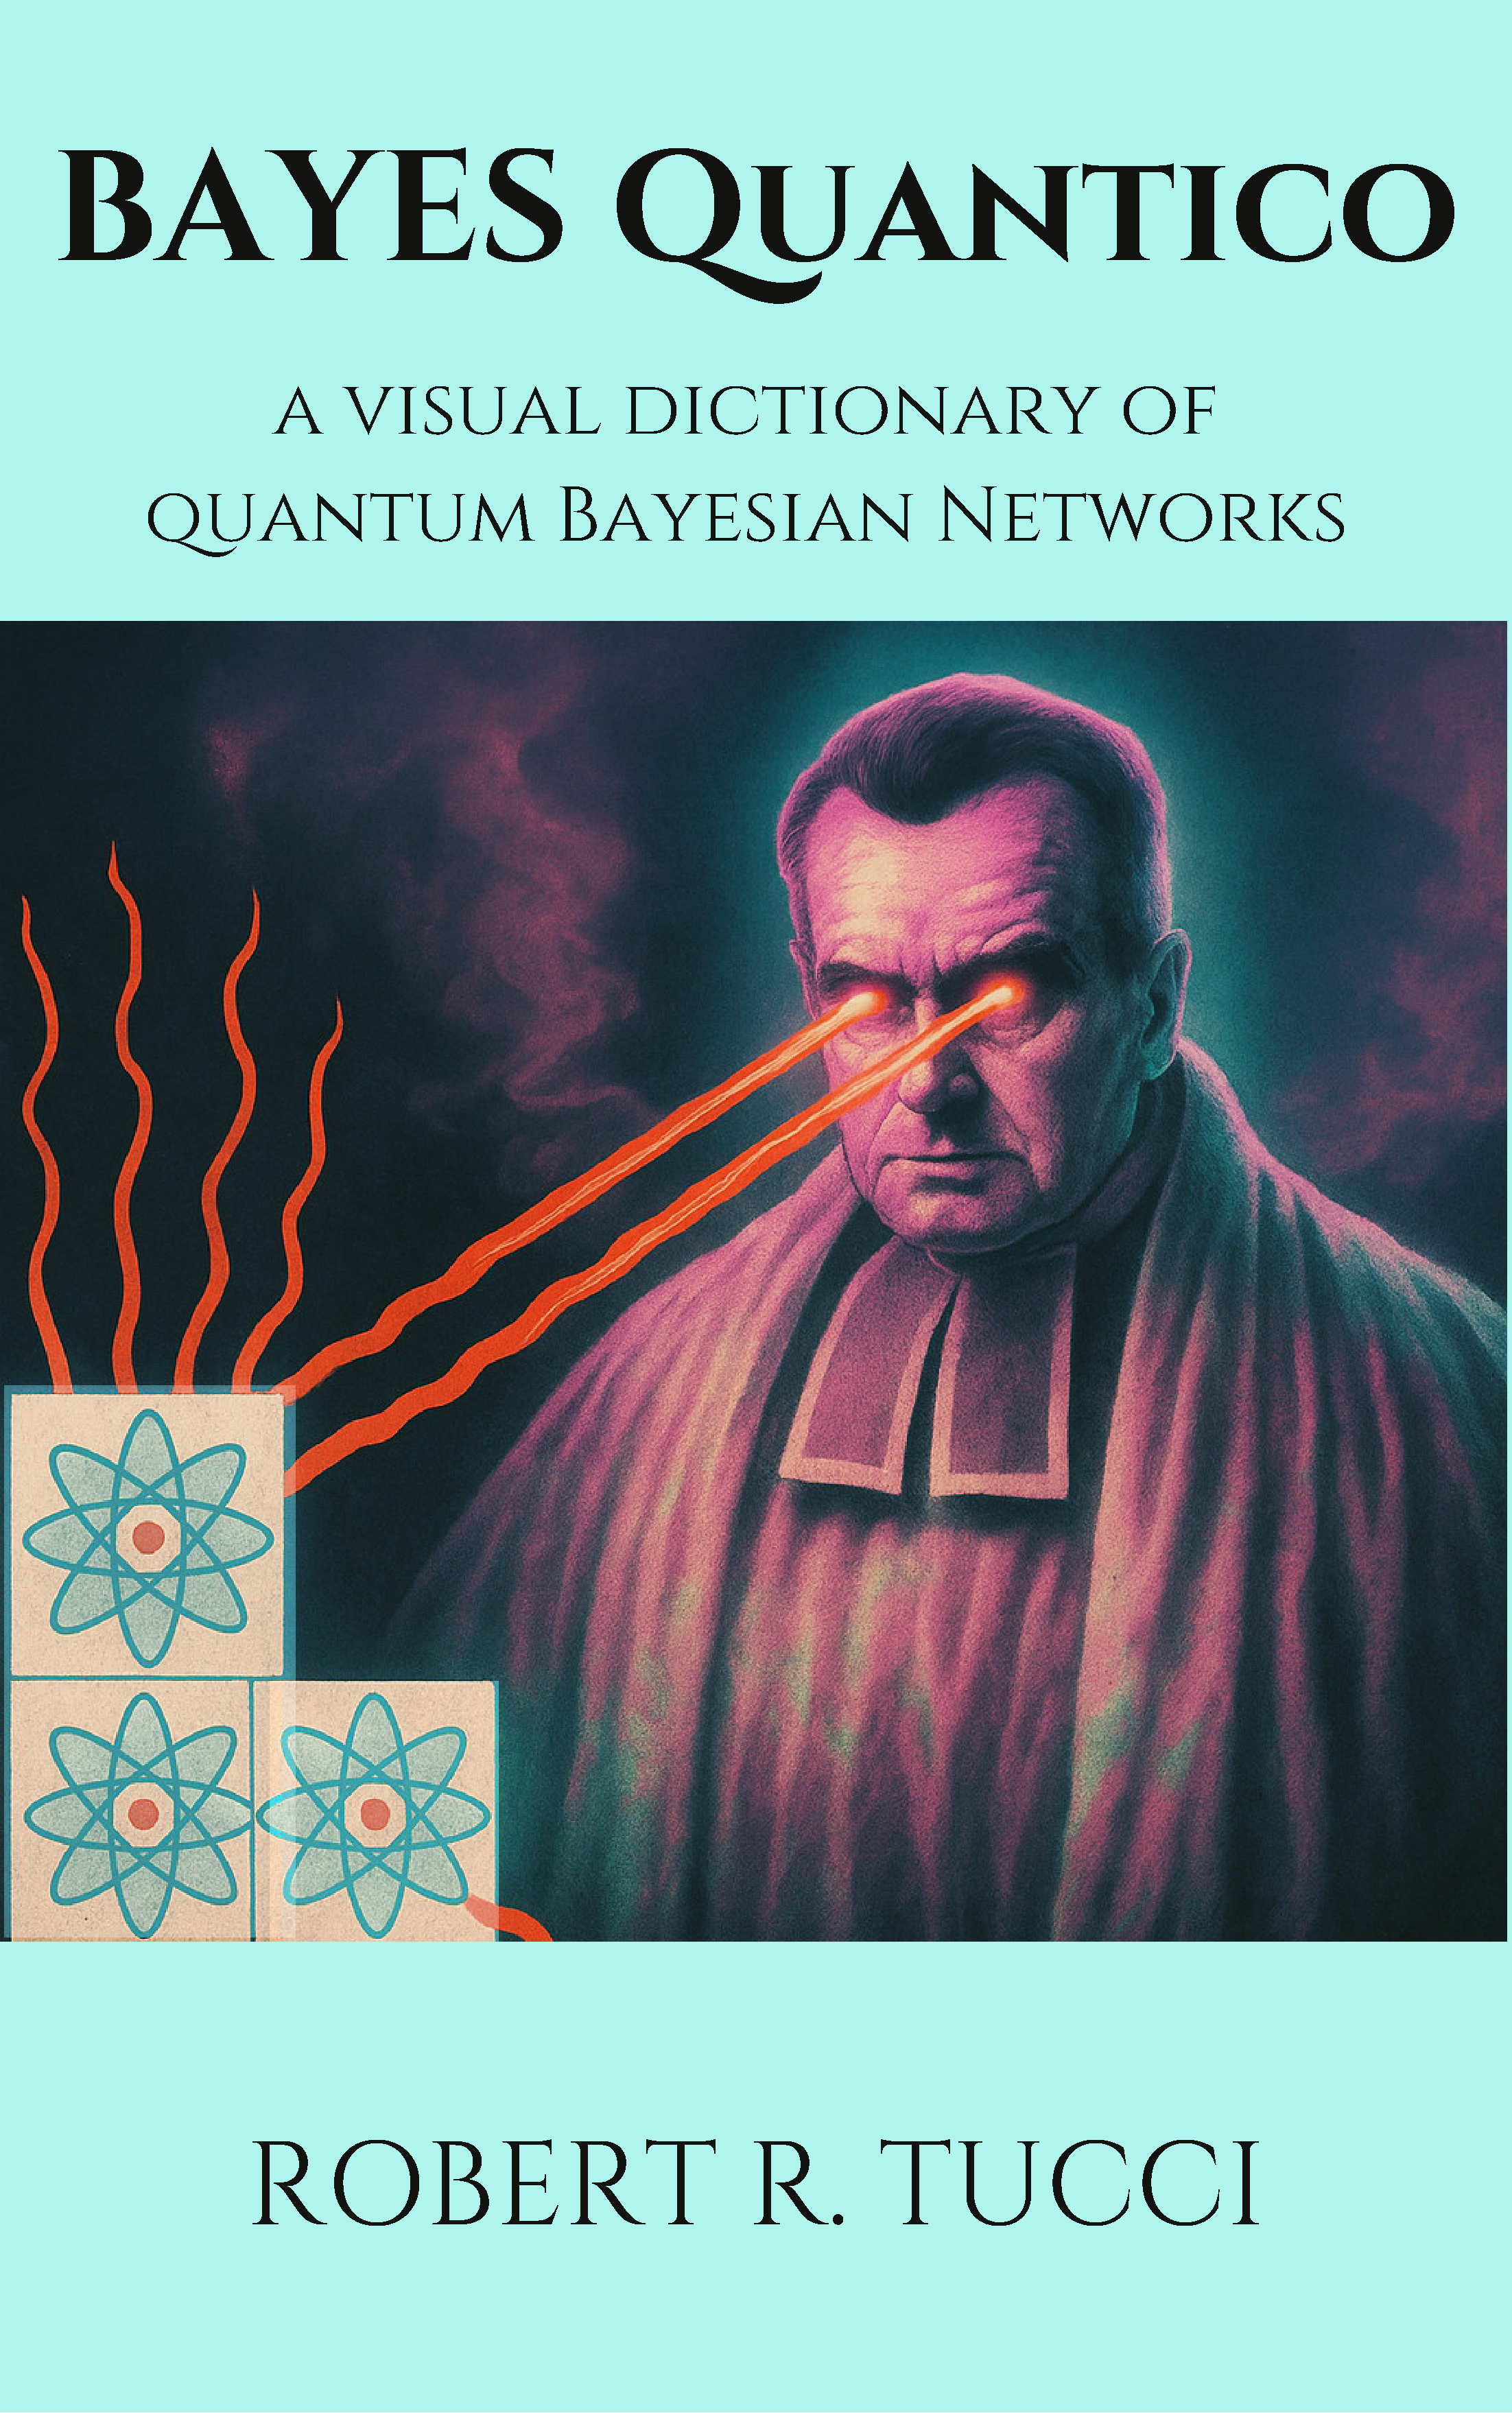
\includepdf[pages=-]{bayes-quantico-cover.pdf}
\maketitle
\newpage
\noindent
{\bf Bayes Quantico}\\
by Robert R. Tucci\\
Copyright \copyright 2025, Robert R. Tucci.\\
\\
This work is licensed under the
Creative Commons Attribution-Noncommercial-No
Derivative Works 3.0 United States License.
 To view a copy of this license, visit the link
\url{https://creativecommons.org/licenses/by-nc-nd/3.0/}
or send a letter to Creative Commons,
 PO Box 1866, Mountain View, CA 94042.
\newpage



\newpage
\setcounter{tocdepth}{10}
\tableofcontents
\chapter{Antisymmetrization: COMING SOON}
\label{ch-antisym}
\chapter{Clebsch-Gordan Coefficients}
\label{ch-clebsch-gordan}
This chapter is based on
Cvitanovic's Birdtracks book Ref.\cite{birdtracks-book}.

Recall that if $\ket{x}$ for
$x\in val(\rvx)$ is a complete, orthonormal
basis in Quantum Mechanics, then

\beq
\av{x|y} =  \delta(x, y)
\quad
\text{(orthonormality)}
\eeq
and

\beq
\sum_x \ket{x}\bra{x} = 1
\quad
\text{(completeness)}
\eeq
Furthermore, if we define

\beq
\pi_x = \ket{x}\bra{x}
\eeq
then $\pi_x$ is a
is a projection operator so

\beq
\pi_x\pi_x=\pi_x
\eeq
and

\beq
\pi_x \ket{y}=  \ket{y}
\delta(x, y),\quad
\bra{y}\pi_x = \bra{y}
\delta(x, y)
\eeq

Below, we will
define matrices $C_\lam$ and $C^\dagger_\lam = D_\lam$.
If we identify $C_\lam$
with $\bra{x}$,
and $C^\dagger_\lam=D_\lam$
with
$\ket{x}$\footnote{
As a mnemonic, I like to think of 
$C_\lam$ as a rounded 
out bra $\bra{x}$
and of $C^\dagger_\lam=D_\lam$
as a rounded out  $\ket{x}$},
then $C_\lam$ and $D_\lam$
satisfy identities
similar to those satisfied by $\bra{x}$ and $\ket{x}$. 
We will show this
in this chapter.



Suppose that  $M\in\CC^{d\times d}$ is a Hermitian matrix. Then we have

\beq
M = D \Lam C
\eeq
where 
$C\in \CC^{d\times d}$ is a unitary matrix, $D=C^\dagger$, and $\Lam$ is a diagonal matrix.



One can partition 
$C$ into rectangular submatrices $C_\lam$ that have  $d_\lam$ rows with $d_\lam < d$, 
such that we have one $C_\lam$
for each eigenvalue $\lam$ of $C$.
Likewise, we can partition 
$D$ into rectangular submatrices $C^\dagger_\lam$ that have $d_\lam$ columns with $d_\lam < d$, such that we have one $D_\lam$
for each eigenvalue $\lam$ of $C$. Thus, if $I^{d_\lam\times d_\lam}$
is the $d_\lam\times d_\lam$
identity matrix,

\beq
\left[
\begin{array}{c}
0
\\
C_\lam^{d_\lam\times d}
\\
0
\end{array}
\right]^{d \times d}
=
\underbrace{\left[
\begin{array}{ccc}
0
&0
&0
\\
0
&I^{d_\lam\times d_\lam}
&0
\\
0
&0
&0
\end{array}
\right]^{d\times d}}_{\pi_\lam}
C^{d\times d}
\eeq
\beq
\left[
\begin{array}{ccc}
0
&(D_\lam)^{d\times d_\lam}
&0
\end{array}
\right]^{d \times d}
=
(D)^{d\times d}
\underbrace{\left[
\begin{array}{ccc}
0
&0
&0
\\
0
&I^{d_\lam\times d_\lam}
&0
\\
0
&0
&0
\end{array}
\right]^{d\times d}}_{\pi_\lam}
\eeq
The matrices $C_\lam$
are called the {\bf Clebsch-Gordan (CG) coefficients} for $M$.

The matrices $\pi_\lam$  
obviously form a complete orthogonal set of projection
operators:

\beq
\sum_\lam \pi_\lam =1,
\quad
\pi_\lam\pi_\mu = \pi_\lam\delta(\lam, \mu)
\eeq
We now have

\beq
\pi_\lam C= \pi_\lam C_\lam,\quad
D \pi_\lam = 
D_\lam \pi_\lam
\eeq

\beqa
C_\lam  D_\lam &=&
\pi_\lam C D \pi_\lam
\\
&=&
\pi_\lam
\eeqa


\beqa
M &=& D \Lam C
\\
&=& 
D\left(\sum_\lam \lam \pi_\lam 
\right)C
\\
&=&\sum_\lam
\lam D_\lam
C_\lam
\eeqa

\beqa
I^{d\times d} &=&
D C
\\
&=&
 \sum_\lam D \pi_\lam C
\\
&=&
 \sum_\lam  \underbrace {D_\lam  C_\lam}_{P_\lam}
\label{eq-cb-series-simple}
\eeqa
We will call Eq.(\ref{eq-cb-series-simple}) the {\bf Clebsch-Gordan (CG) series}
for $M$.

Note that
 $C_\lam^\dag C_\lam\neq \pi_\lam$ whereas $C_\lam D_\lam = \pi_\lam$.
However, 

\beq
1 =\sum_\lam D_\lam C_\lam=
\sum_\lam \underbrace{C_\lam D_\lam}_{\pi_\lam}
\eeq

If we define

\beq
P_\lam = D_\lam C_\lam=
D\pi_\lam C
\eeq
then the $P_\lam$ form a complete orthogonal set of
projection operators, just like the $\pi_\lam$.

\beq
\sum_\lam P_\lam =1,
\quad
P_\lam P_\mu =
P_\lam \delta(\mu, \nu)
\eeq
Whereas the $\pi_\lam$ satisfy

\beq
\pi_\lam C= \pi_\lam C_\lam,\quad
D \pi_\lam = 
D_\lam \pi_\lam
\eeq
the $P_\lam$ satisfy

\beq
CP_\lam= C_\lam P_\lam ,\quad
P_\lam D  = 
P_\lam D_\lam
\eeq

Since we are assuming $M$ is Hermitian,
its eigenvalues are real. 
Thus, we can absorb
the eigenvalue $\lam$ into the CG
coefficients   by defining

\beq
\calc_\lam =\sqrt{\lam}C_\lam
\eeq
and writing

\beq
M= \sum_\lam \calc^\dagger_\lam \calc_\lam
\eeq



Let $b^{:nb}=(b_1, b_2, \ldots, b_{nb})$ where $b_i\in Z_{[0,d_{\mu_i}]}$  and $a\in Z_{[1,d_\lam]}$.
Assume that

\beq
d_\lam = \prod_{i=1}^{:nb}d_{\mu_i}
\eeq

Now define the birdtracks


\beq
(C_\lam)\indices{
_{a}^{rev(b^{:nb})}
}=
\bcen
\xymatrix@C=1pc@R=1pc{
&&\mu_1 b_1\ar[dl]
\\
\lam a
& C_\lam\ar@[green][l]
&\mu_2 b_2\ar[l]
\\
&&\mu_{nb} b_{nb}\ar[lu]
}
\ecen
\eeq
and



\beq
(D_\lam)
\indices{
^{a}_{b^{:nb}}
}=
\bcen
\xymatrix@C=1pc@R=1pc{
\mu_1 b_1
\\
\mu_2 b_2
&(D_\lam)
\ar[lu]\ar[l]\ar[ld]
&\lam a\ar@[green][l]
\\
\mu_{nb} b_{nb}
}
\ecen
\eeq
 We will
assume  there is no
difference
between when a Greek letter is lowered 
and when it is  raised. Also, all summations over a Greek letter will be 
stated explicitly;
i.e., no implicit summations
over repeated Greek letters.

On the other hand, the Latin letter indices $b_i, a$ of $C_\lam$
and $D_\lam$
may be lowered or raised and their arrows
changed from outgoing to  incoming or vice versa. Furthermore,
we will use implicit
summation over
repeated Latin letters.

The Greek letters label representation
of the group (not necessarily irreps).
Each $b_i$ 
labels a member
of $\mu_i$, and
each $a$ labels
a member of $\lam$.


\beq
\begin{array}{l}
\myboxed{
(C_\lam)\indices{
_a
^{rev((b')^{:nb})}
}
(P_\mu)\indices{
_{(b')^{:nb}} 
^{rev(b^{:nb})}
}=
\delta(\mu,\lam) 
(C_\mu)\indices{
_a
^{rev(b^{:nb})}
}
,\quad
C_\lam P_\mu =
\delta(\mu,\lam) C_\mu}
\\
\bcen
\xymatrix@C=1pc@R=1pc{
&
&\sum b'_1\ar[dl]
\\
a& C_\lam\ar[l]
&\sum b'_2\ar[l]
\\
&
&\sum b'_{nb}\ar[lu]
}
\xymatrix@C=1pc@R=1pc{
&
&b_1\ar[ld]
\\
&P_\mu\ar[l]
\ar[ld]\ar[lu]
&b_2
\ar[l]
\\
&
&b_{nb}\ar[lu]
}
\ecen
=
\delta(\mu, \lam)
\bcen
\xymatrix@C=1pc@R=1pc{
&
&b_1\ar[dl]
\\
a& C_\lam\ar[l]
&b_2\ar[l]
\\
&
&b_{nb}\ar[lu]
}
\ecen
\end{array}
\eeq


\beq
\begin{array}{l}
\myboxed{
(P_\mu)\indices{
_{b^{:nb}}
^{rev((b')^{:nb})}
}
(D_\lam)\indices{
^a
_{(b')^{:nb}}
}=
\delta(\mu, \lam) 
(D_\mu)\indices{
^a
_{b^{:nb}}
}
,\quad
P_\mu D_\lam=
\delta(\mu, \lam) D_\mu}
\\
\bcen
\xymatrix@C=1pc@R=1pc{
b_1
&
&\sum b'_1\ar[ld]
\\
b_2
&P_\mu\ar[l]
\ar[ld]\ar[lu]
&\sum b'_2
\ar[l]
\\
b_{nb}
&
&\sum b'_{nb}\ar[lu]
}
\ecen\bcen
\xymatrix@C=1pc@R=2pc{
\\
&(D_\lam)
\ar[lu]\ar[l]\ar[ld]
& a\ar[l]
\\
&
}
\ecen
=
\delta(\mu, \lam)
\bcen
\xymatrix@C=1pc@R=1pc{
b_1
\\
b_2
&(D_\lam)
\ar[lu]\ar[l]\ar[ld]
& a\ar[l]
\\
b_{nb}
}
\ecen
\end{array}
\eeq





\beq
\begin{array}{l}
\myboxed{
(C_\lam)\indices{
_a
^{rev(b^{:nb})}
} 
(D _\mu)\indices{
^{a'}_{b^{:nb}} 
}
= \delta(\lam, \mu)
\delta_{a}^{a'},
\quad
C_\lam D_\mu =
\delta(\mu, \lam)
}
\\
\bcen
\xymatrix@C=1pc@R=1pc{
&&\sum b_1\ar[dl]
\\
a
& C_\lam\ar[l]
&
\sum b_2\ar[l]
\\
&&\sum b_{nb}\ar[lu]
}
\xymatrix@C=1pc@R=1pc{
\\
&(D_\mu)
\ar[lu]\ar[l]\ar[ld]
& a'\ar[l]
\\
&
}
\ecen =
\delta(\mu, \lam)
\xymatrix{
a
&a'
\ar[l]|\bullet
}
\end{array}\eeq

\beq
\begin{array}{l}
\myboxed{
\sum_\lam
(D_\lam)\indices{
^a
_{b^{:nb}}
}
(C_\lam)
\indices{_a
^{rev((b')^{:nb})}
}=
\delta^{rev((b')^{:nb})}_{b^{:nb}}
,\quad
\sum_\lam D_\lam C_\lam = 1
}
\\
\sum_\lam
\bcen
\xymatrix@C=1pc@R=1pc{
b_1
\\
b_2
&(D_\lam)
\ar[lu]\ar[l]\ar[ld]
& \sum a\ar[l]
\\
b_{nb}}
\xymatrix@C=1pc@R=1pc{
&
&b'_1\ar[dl]
\\
& C_\lam\ar[l]
&b'_2\ar[l]
\\
&
&b'_{nb}\ar[lu]
}
\ecen
=
\bcen
\xymatrix@C=1pc@R=1pc{
b_1
&\bullet
&b'_1\ar[ll]
\\
b_2
&\bullet
&b'_2
\ar[ll]
\\
b_{nb}
&\bullet
&b'_{nb}\ar[ll]
}
\ecen
\end{array}
\eeq


\chapter{Invariants}
\label{ch-invariants}
\chapter{Spectral Decomposition and Eigenvalue Projection Operators: COMING SOON}
\label{ch-spectral-decom}

$M\in \CC^{d\times d }$

\beq
M\ket{v}=\lam \ket{v}
\eeq
If $M$ is Hermitian ($H^\dagger=H$), its eigenvalues are real. ( $\lam =
\av{\lam|M\lam}\in\RR$)


\beq
cp(\lam)\eqdef \det(M-\lam)=0
\eeq

If $M$ is a Hermitain  matrix, then there exists
a unitary matric ($CC^\dagger = C^\dagger C =1$)
such that

\beq
CMC^\dagger=
\left[
\begin{array}{cccc}
D_{\lam_1}
&0
&0
&0
\\
0
&D_{\lam_2}
&0
&0
\\
0
&0
&\ddots
&0
\\
0
&0
&0
&D_{\lam_r}
\end{array}
\right]
\eeq
where

\beq
D_{\lam_i} =
\text{diag}\underbrace{(\lam_i,\lam_i, \dots,\lam_i)}_{d_i\text{ times}}
\eeq

\beq
d=\sum_{i=1}^r d_i
\eeq


\beq
CMC^\dagger =
\left[
\begin{array}{cc}
\lam_1 &0
\\
0&\lam_2
\end{array}
\right]
\eeq

\beq
C P_1 C^\dagger=
\left[
\begin{array}{cc}
1&0
\\
0&0
\end{array}
\right]
=
\frac{CMC^\dagger -\lam_2}{\lam_1-\lam_2}
\eeq

\beq
CP_2 C^\dagger =
\left[
\begin{array}{cc}
0&0
\\
0&1
\end{array}
\right]
=
\frac{CMC^\dagger-\lam_1}{\lam_2-\lam_1}
\eeq

If $I^{d_i\times d_i}$
is the $d_i$
dimensional unit matrix,
\beqa
P_i &=&
C^\dagger
diag(0,\ldots,0, I^{d_i\times d_i},0, \dots, 0)C
\\
&=&
\prod_{j\neq i}
\frac{M -\lam_j}{\lam_i -\lam_j}
\eeqa

Note that $P_i$ are Hermitian
($P_i^\dagger = P_i$)
because $M$
is Hermitian and
its eigenvalues are real.)

Note that
$P_i$ and $M$
commute

\beq
[P_i, M]=
P_iM-MP_i=0
\eeq

orthogonal
\beq
P_i P_j =\delta(i,j)P_j
\eeq

complete
\beq
\sum_i P_i =1
\eeq

\beq
M= \sum_{i=1}^r
P_iM P_i
\eeq

\beq
d_i = \tr P_i
\eeq

\beqa
CMP_1C^\dagger &=&
\left[
\begin{array}{cc}
\lam_1&0
\\
0&\lam_2
\end{array}
\right] 
\left[
\begin{array}{cc}
1&0
\\
0&0
\end{array}
\right] 
\\
&=&
\lam_1
\left[
\begin{array}{cc}
1&0
\\
0&0
\end{array}
\right] 
\eeqa

\beq
MP_i = \lam_i P_i \;
\text{(no $i$ sum)}
\eeq

\beq
f(M) P_i = f(\lam_i)P_i \;
\text{(no $i$ sum)}
\eeq

$M^{(1)}, M^{(2)}$

\beq
[M^{(1)}, M^{(2)}]  =0
\eeq
Use $M^{(1)}$ to decompose $V$
into $\bigoplus_i V_i$.
Use  $M^{(2)}$ to decompose $V_i$ into
$\bigoplus_j V_{i,j}$. 
If $M^{(1)}$ and $M^{(2)}$ don't
commute, let $P^{(1)}_i$ be the eigenvalue 
projection operators of $M^{(1)}$. The replace $M^{(2)}$ by $P^{(1)}_i M^{(2)}P_i^{(1)}$

\beq
[M^{(1)}, P^{(1)}_iM^{(2)}P^{(1)}_i]  =0
\eeq




\chapter{Sp(n)}
\label{ch-sp-n}
\chapter{SO(n)}
\label{ch-so-n}
\chapter{SU(n)}
\label{ch-su-n}
\chapter{Symmetrization: COMING SOON}
\label{ch-sym}

%symmetrizer
\xymatrix@R=.5pc{
a
&\cals\ar@2{-}[dd]\ar@{-}[l]
&x\ar@{-}[l]
\\
b&\ar@{-}[l]
&y\ar@{-}[l]
\\
c&\ar@{-}[l]
&z\ar@{-}[l]
}
\chapter{Tensor and Diagrammatic Notation: COMING SOON}
\label{ch-tensor-dia-not}
\beqa
P(y) &=&\sum_x P(y|x)P(x)
\\
\av{y|\psi} &=& \sum_x \underbrace{\av{y|A|x}}_{A(y|x)}\av{x|\psi}
\eeqa

\beq
\xymatrix{&\ar[l]}=\xymatrix{&\ar[l]^{\sum a}} =\sum_a \ket{a}\bra{a}
\eeq

\beqa
\av{a|q} &=& \sum_b\av{a|G|b}\av{b|q}
\\
q_a &=&  \sum_b G^b_a q_b
\\
\xymatrix{
&q\ar[l]^a}
&=&
\xymatrix{&G\ar[l]^a & q\ar[l]^{\Sigma b}
}
\eeqa




\beqa
\av{q|a} &=& \sum_b\av{b|G^\dagger|a}\av{q|b}
\\
q^a &=&  \sum_b (G^\dagger)_b^a q^b
\\
\xymatrix{
q&\ar[l]^a}
&=&
\xymatrix{q&G^\dagger\ar[l]^{\sum b}&\ar[l]^a
}
\eeqa

\beq\xymatrix{
&q\ar[l]^a}
=
\xymatrix{a&q\ar[l]}
\eeq

\beq\xymatrix{
q&\ar[l]^a}
=
\xymatrix{
q&a\ar[l]
}\eeq

\beq
G_{a,b,c}^{d,e} = \av{a,b,c|G| d,e} =
\xymatrix{a & G\ar[l]\ar[ld]\ar[ldd] & d\ar[l]
\\
b&&e\ar[lu]
\\
c}
\eeq

\beqa
\av{b_1, b_2|h|a_1, a_2}
&=&
\av{G^\dagger b_1, G^\dagger b_2|h|Ga_1, Ga_2}
\\
\xymatrix{
a_1\ar[dr]
&&a_2\ar[dl]
\\
&h\ar[dl]\ar[dr]
\\
b_1 & & b_2
}
&=&
\xymatrix@R=15pt{
a_1\ar[d]
&&a_2\ar[d]
\\
G \ar[dr]
&& G\ar[dl]
\\
&h\ar[dl]\ar[dr]
\\
G^\dagger \ar[d]
&& G^\dagger \ar[d]
\\
b_1 & & b_2
}
\eeqa

\beqa
G_b^a &=& \delta_b^a + i\sum_j\eps_j
(T_j)_b^a
\\
\xymatrix{&G\ar[l]^b&\ar[l]^a}
&=&
\xymatrix{&\delta\ar[l]^b&\ar[l]^a}
+i\sum_j\eps_j
\xymatrix{&T_j\ar[l]^b&\ar[l]^a}
\eeqa
Assume $T^\dagger_j = T_j$.
To first order in $\eps_j$, 
\beqa
0
 &=& i\sum_j \eps_j
\left(\begin{array}{c}
\xymatrix@R=15pt{
a_1\ar[d]
&&a_2\ar[d]
\\
T_j \ar[dr]
&& \delta\ar[dl]
\\
&h\ar[dl]\ar[dr]
\\
\delta \ar[d]
&& \delta \ar[d]
\\
b_1 & & b_2
}  \xymatrix{\\
\\+}
\xymatrix@R=15pt{
a_1\ar[d]
&&a_2\ar[d]
\\
\delta \ar[dr]
&& T_j\ar[dl]
\\
&h\ar[dl]\ar[dr]
\\
\delta \ar[d]
&&\delta \ar[d]
\\
b_1 & & b_2
}
\end{array}
 \right)
 \\
 &-& i\sum_j \eps_j
\left(\begin{array}{c}
\xymatrix@R=15pt{
a_1\ar[d]
&&a_2\ar[d]
\\
\delta \ar[dr]
&& \delta\ar[dl]
\\
&h\ar[dl]\ar[dr]
\\
T_j \ar[d]
&& \delta \ar[d]
\\
b_1 & & b_2
}  \xymatrix{\\
\\+}
\xymatrix@R=15pt{
a_1\ar[d]
&&a_2\ar[d]
\\
\delta \ar[dr]
&& \delta\ar[dl]
\\
&h\ar[dl]\ar[dr]
\\
\delta \ar[d]
&&T_j \ar[d]
\\
b_1 & & b_2
}
\end{array}
 \right)
\eeqa
from which we get one equation for each $\eps_j$.



\bibliographystyle{plain}
\bibliography{references}
\end{document}

